%
% File acl2013.tex
%
% Contact  navigli@di.uniroma1.it
%%
%% Based on the style files for ACL-2012, which were, in turn,
%% based on the style files for ACL-2011, which were, in turn, 
%% based on the style files for ACL-2010, which were, in turn, 
%% based on the style files for ACL-IJCNLP-2009, which were, in turn,
%% based on the style files for EACL-2009 and IJCNLP-2008...

%% Based on the style files for EACL 2006 by 
%%e.agirre@ehu.es or Sergi.Balari@uab.es
%% and that of ACL 08 by Joakim Nivre and Noah Smith

\documentclass[11pt]{article}
\usepackage{acl2013}
\usepackage{times}
\usepackage{url}
\usepackage{latexsym}
\usepackage{graphicx}
%\setlength\titlebox{6.5cm}    % You can expand the title box if you
% really have to

\title{Scaling Dependency-Based Compositional Semantics to a Wide Domain}

\author{Amelia Harrison \\
  Department of Computer Science\\
  University of Texas at Austin \\
  {\tt ameliaj@cs.utexas.edu} \\\And
  Subhashini Venugopalan \\
  Department of Computer Science\\
  University of Texas at Austin \\
  {\tt vsubhashini@cs.utexas.edu} \\}

\date{}

\begin{document}
\maketitle
\begin{abstract}
   Recent work in semantic parsing for compositional question answering has shown
that this task can be successfully approached using question-answer pairs rather
than questions annotated with logical forms for training. However, existing
datasets for this task are relatively small. It is unclear  that any existing
approaches to compositional question answering can scale to larger datasets or
datasets with wide coverage, even without the burden of producing logical 
forms for training.  In this paper, we explore the possibility of scaling 
the approach presented in \cite{LJK11} to a larger dataset with wider coverage. 

\end{abstract}

\section{Introduction}

The semantic parsing task addressed in this paper is that of
answering compositional natural language questions given a database which is 
assumed to contain sufficient information to derive an answer. The {\sc geo}
dataset has historically been used for this task. State-of-the-art systems can
answer the compositional questions given in the {\sc geo} dataset with fairly
high accuracy. 

In recent work, Liang et al. present a novel approach to the semantic parsing
task. Most prior approaches have focused on training parsing models using natural
language utterances annotated with logical forms.\footnote{\cite{CGCR10}, 
\cite{CGRR11}, and \cite{PD09} are notable exceptions.} In this work, however,
the logical forms are treated as latent variables, and a semantic parsing model
is trained using natural language questions and their corresponding answers. 
This sort of ``weak supervision'' is advantageous because obtaining 
logical forms for natural language utterances requires expert annotators and is
thus quite costly. This work is notable because it takes this weakly supervised 
approach, and also because it introduces an new formalism called
dependency-based compositional semantics (DCS) trees for representing 
the meaning of a natural language question. 

In this paper, we explore the
possibility of applying the DCS framework in a wide-domain setting with a much
larger underlying database. We present a new wide-domain dataset for compositional 
question answering called {\sc infobox}. We identify obvious limitations that prevent 
the unmodified DCS framework from scaling to this dataset. We then show that
those limitations can be lifted, incurring some performance hit, for the {\sc
geo} task. Finally, we present the results of the applying the modified DCS
framework to {\sc infobox}. 

\section{A Wide-Domain Dataset for Compositional Question Answering}

The dataset we present, {\sc infobox}, is very similar in spirit to {\sc geo}, but
covers a much broader domain. It consists of a database and a set of
English questions. Each question is annotated with an answer consistent with 
the facts in the database. The database itself is a subset of the publicly 
available {\sc dbpedia}.\footnote{{\tt http://wiki.dbpedia.org/Downloads38}} 
The whole of {\sc dbpedia} is very large, consisting of about 25 million 
facts. Manipulating so many facts can introduce memory management issues, and
so we use a subset of {\sc dbpedia} for our database. We chose facts with information
about the 30,000 most commonly occurring entities to serve as the
{\sc infobox} database. This yielded a database containing about 672,000 facts,
775 distinct \emph{relational predicates} and 171 distinct \emph{type predicates}.
We use the term relational predicates to refer to binary predicates that express
a relation between entities. Type predicates are unary predicates that express
ontological information about an entity. All of the predicates in the {\sc infobox}
databse are either binary or unary.  (For comparison, the {\sc geo} database 
contains about Z 
facts and Z distinct predicates.) We then manually produced a set of 
150 question-answer pairs. Many of the
questions are compositional in the sense that they require aggregating
information from multiple facts. 

Table \ref{tb} shows examples of the questions in {\sc infobox}. It is worth noting,
that we originally hypothesized that using the DCS framework would remove the 
burden of producing annotated logical forms and thereby make producing a large
body of questions much easier. When we began to construct {\sc infobox}, however, we
realized that it is essential that the question-answer pairs be consistent with 
the given database in order to learn to answer questions using DCS. Without
directly consulting the database while drafting answers, it is easy to produce
answers that are not consistent with the database. One might provide answers
that differ in spelling or phrasing, or alternatively provide an answer
altogether different from the answer the database would provide. Accordingly, 
in order to ensure that the answers we provided were correct, we still had to produce a
database query corresponding to each question. 
\begin{center}
\begin{table*}[ht]
{\small
\hfill{}
\begin{tabular}{|l l|}
\hline
    &\\
    Q: In which city was the author of {\emph Tarzan} born? & A: Chicago. \\&\\
    Q: What is the currency of the country with the capital 
       Kampala? & A: Ugandan shilling. \\ &\\ 
    Q: How many instruments does the San Francisco born Metallica band member
       play? & A: 4. \\&\\  
    Q: What state was Upton Sinclair born in? & A: Maryland. \\&\\
\hline
\end{tabular}}
\hfill{}
\caption{Questions from {\sc infobox}}
\label{tb}
\end{table*}
\end{center}
\section{Background and Limitations of the DCS Framework} 
There is one obvious limitation in the DCS framework that might hinder attempts
to bring this work to scale on a wide-domain dataset.  Here, we provide a brief 
overview of DCS and explain its major limitation. We then explain our approach
to addressing this limitation. 

\subsection{Background}

Liang et al. propose a novel logical form, called DCS trees, for representing the 
meaning of a natural language question. A DCS tree is designed to closely mirror
the syntactic dependency parse of a natural language utterance. Nodes in the
tree correspond to predicates in the database, and each edge corresponds to one of
a fixed set of ``relations''. Although the structure of a tree reflects that of
the dependency parse of the utterance it represents, the semantics of the relations 
associated with the edges are powerful enough to allow for divergence between
syntactic and semantic scope. This makes DCS a more expressive
logical language than {\sc FunQL} \cite{KWM05}. Like an {\sc SQL} or
{\sc FunQL} query, a DCS tree can be evaluated with respect to a database to 
produce an answer.  

In the DCS framework, each natural language question is associated with a 
number of permissible DCS trees -- that is DCS trees 
which may correspond to the actual meaning of the utterance, and in turn
evaluate to the correct answer. The set of permissible trees is determined, 
in part, by a fixed set of {\it lexical
triggers}. A lexical trigger associates a word or sequence of words with a
predicate in the database. Roughly speaking, the set of permissible trees is
then formed by identifying all syntactically correct ways of combining the
predicates triggered by the words in an utterance, using the relations available. 
Clearly, the success of this model depends crucially on the set of lexical
triggers. In \cite{LJK11}, two sets of lexical triggers are evaluated, $L$ and
$L^+$.  In $L$, each predicate has an associated set of  POS-tags, and each word
in a question is POS-tagged. A given word then triggers all predicates whose 
associated POS-tags include that assigned to the word. In $L^+$, many predicates
are manually associated with a ``prototype'' word. The prototype words then
trigger only the predicates with which they have been manually associated and do
not trigger any predicates based on their POS-tags. Words that are not prototype
words still trigger predicates based on their POS-tags. Both $L$ and $L^+$ also
include a small set of general manually specified triggers for function words and 
a set of ``trace predicates''. Trace predicates are those that can be inserted without 
any overt lexical trigger.   

Learning in the DCS framework uses a discriminative model which places a
probability distribution over
all of the permissible DCS trees for a given natural language utterance. The
model features are indicators of various relationships between the utterance and
the candidate tree. For example, one type of feature indicates that a given word
triggers a given predicate. The model is trained using an EM-like algorithm
which attempts to find the feature weights that maximize the number of questions
whose top-weighted DCS tree evaluates to the specified answer. 

Evaluating on the {\sc Geo} and {\sc Jobs} datasets, the model presented in
\cite{LJK11} using the lexical trigger set $L^+$ outperforms all previous systems.  
Even using the more rudimentary lexical trigger set $L$, the model achieves
recall comparable to the best previous system (that of Kwiatkowski et al.
\cite{KZGS10}), which utilizes logical form annotations.  

\subsection{Limitations} 

There is one notable aspect of the DCS framework which requires nontrivial 
supervision: identifying the set of lexical triggers. 
Even the base set of lexical triggers $L$, used in
\cite{LJK11} required annotating the predicates with the POS-tags that should
trigger them. This is not such a daunting task for the {\sc Geo} dataset which
includes only about 30 predicates. However, if we try to extend the system to
{\sc infobox}, the time investment required for specifying lexical triggers 
suddenly becomes quite significant. Using POS-tagged based triggers for {\sc
infobox} is also unrealistic because of the number of distinct predicates in the
database. Lexical triggers play the role of reducing the number of possible DCS
trees that a question can generate. However, if each word is associated with a
very large number of predicates the permissible set of DCS trees will be
correspondingly large.  

\section{Automatically Generating Lexical Triggers}

We alleviate the burden of hand-crafting a set of lexical triggers by taking
advantage of predicate names and the values associated with predicates. 
 
\subsection{Lexical Triggers for {\sc geo}}
Our approach for the {\sc geo} dataset depends entirely on predicate names. 
Admittedly, the predicates in a database
may not be informatively named. Furthermore, this approach eliminates the
possibility of a language independent system. We assume that predicates have
informative English names. For the {\sc geo} dataset, this assumption
for the most part holds.  We explore a method for automatically generating 
lexical triggers using WaCkypedia.
\footnote{http://wacky.sslmit.unibo.it/doku.php?id=corpora} We construct 
a list of words most commonly occurring in the same sentence as words in the predicate 
names. For a given predicate, we then use the words in WaCkypedia with which its 
constituent words most commonly co-occur, removing stop words. 
 
\subsection{Lexical Triggers for {\sc infobox}}
For the {\sc infobox} dataset we also use lexical triggers
extracted from WaCkypedia. However, with this 
dataset we attempted to make our lexical trigger generation approach not 
depend on the assumption that predicate names are in English and informative.

Rather than
using the words that most commonly co-occur with the words in a predicate name, we
use the words that most commonly co-occur with the co-occur with the set of
values associated with a given predicate. For example, the relational predicate
{\bf mascot} occurs in the facts {\bf mascot}(\emph{Arizona State University},
\emph{Sparky}) and {\bf mascot}(\emph{California Institute of Technology},
\emph{Beaver}), among others. To construct the lexical trigger set for {\bf
mascot} we take the words that most commonly co-occur with both 
\emph{Arizona State University} and \emph{Sparky} or any other value pairs
for the predicate {\bf mascot}. Again, we remove stop words. The top results for
the {\bf mascot} predicate are ``university'', ``school'', and ``mascot.''

This predicate-name-independent approach was possible for the {\sc infobox} 
dataset because of the very regular structure of the database. (Recall that the
{\sc infobox} database contains only binary relational predicates and unary type
predicates.) Such an approach was not applicable for the {\sc geo} database on
the other hand because the predicates in that database have widely varying
arities.  

\section{Evaluation and Results}\label{results}

We perform two sets of experiments: one to evaluate the effectiveness of our
automatically generated lexical trigger sets for the {\sc geo} dataset, and
one to test our approach on the {\sc infobox} dataset. 

\subsection{Experiments for the {\sc geo} dataset}

\begin{figure}[!htb]\label{fig1}
\begin{center}
  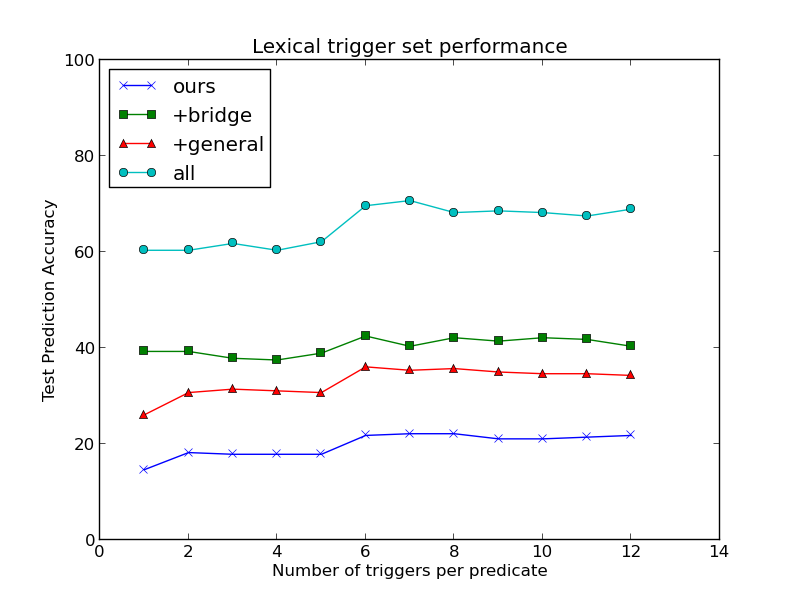
\includegraphics[scale=0.40]{figs/ablationTest.png}
\caption{Graph showing the effect of varying the number of lexical triggers per predicate 
on {\sc geo}. }
\end{center}
\end{figure}

The code that implements \cite{LJK11} is publicly
available.\footnote{http://cs.stanford.edu/~pliang/papers/} We use this
implementation, and replace the trigger sets $L$ and $L^+$, with our own
automatically generated trigger sets. We do experiments with and without the
general functional triggers and trace predicates from \cite{LJK11}, and varying
the number of lexical triggers included for each predicate. All of our
experiments use the {\sc geo} dataset with 880 questions and an 80/20 train/test
split. 

Figure \ref{fig1} shows the test prediction accuracy (i.e. the percentage of
test questions answered correctly) for each trigger set.  
The line labeled ``ours'' shows the results using only the
automatically generated triggers. The line labeled ``+bridge'' shows the
results using the generated triggers and the trace predicates from
\cite{LJK11}. The line labeled ``+general'' represents generated triggers and
the general functional predicates from \cite{LJK11}. The line labeled ``all''
represents results when all three sets are included.


\subsection{Experiments for the {\sc infobox} dataset}

We run similar experiments for the {\sc infobox} dataset. Again we use an 80/20
train/test split, and vary the number of automatically generated lexical
triggers used. The test prediction accuracy for this dataset was identically
zero. (See Section \ref{disc} for discussion.) For this reason, we report the
training prediction accuracy as well as the test and training oracle accuracy
for this dataset. 

The training prediction accuracy refers to the percentage of
training questions for which the model produces a correct answer. For any
question input the DCS framework uses the lexical triggers to generate a set of
DCS trees corresponding to possible logical forms for the given question. 
The oracle accuracy refers to the percentage of questions for which a DCS
tree corresponding to a correct answer was among the trees generated by the model.  
Figure \ref{fig2} shows the results. 

\begin{figure}[!htb]\label{fig2}
\begin{center}
  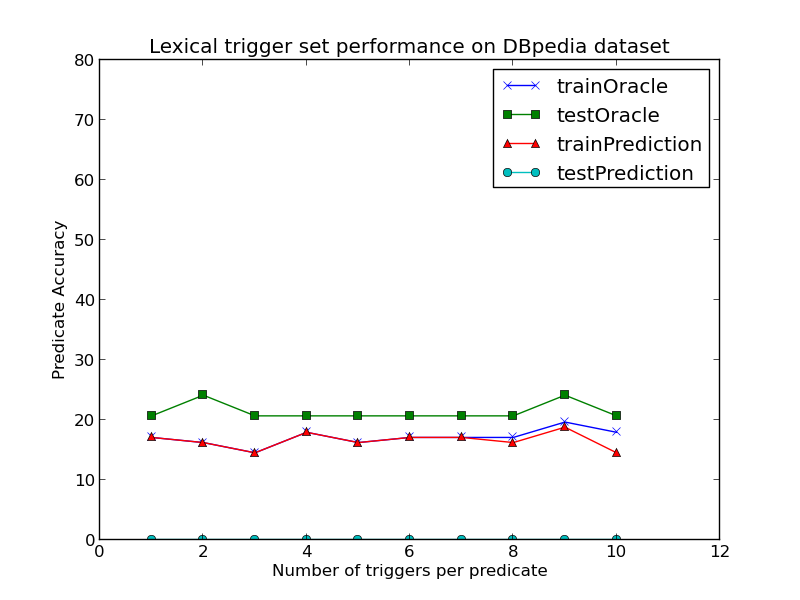
\includegraphics[scale=0.40]{figs/ibPerf.png}
\caption{Performance of automatically generated lexical triggers on the
wide-domain {\sc infobox} dataset.}
\end{center}
\end{figure}

\subsection{Discussion}

The automatically generated trigger sets perform relatively well on the
{\sc geo} dataset. When the trace predicates and general functional triggers are
included, the test prediction accuracy approaches~$.70$. It is worth noting that 
including the trace predicates and general functional triggers is reasonable
because these are independent of the size of the database. It makes sense then,
that we could manually develop a comparable set of trac predicates and
functional triggers for the {\sc infobox} dataset. 

Although the results for our automatcally generated trigger sets
are substantially lower than the best test accuracies reported in
\cite{LThesis} (see Table 2) ,the results do lend some credence to 
the idea that the DCS framework might successfully scale to a wide domain. 

However, the test prediction accuracies for the {\sc infobox} dataset literally
could not be worse. We suspect that the {\sc infobox} is too small to produce
meaningful results. Certainly, as it contains only 150 questions it does not
make sense to try and compare these results to the results on the {\sc geo}
dataset. With more time, we would run the experiments described in the section
above usig only 150 of the {\sc geo} questions. This would allow us to directly
compare the performance of automatically generated lexical triggers across the
two datasets, and give a better idea of the effect of scaling the number of
facts and predicates in the database on performance.   

As Figure 2 shows, in training the oracle and prediction accuracies are
almost uniformly identical. This indicates that the model is overfitting the 
small amount of training data. Although the test oracle accuracy is high, the
learned model does not generalize to the test set. Accordingly, 
the test prediction accuracy results are abysmal.  

\begin{center}
\begin{table}[!h]
\centering
\begin{tabular}{|l|c|c|}
\hline
{\textbf{Lexicon Trigger}} & {\textbf{Test Prediction}} \\ %\cline{4}
\textbf{Set} &  \textbf{Accuracy} \\
%\textbf{Function}& (after iteration 8) &\textbf{words}  & (total)\\
\hline
ours      & {{21.78}} \\ \hline
+bridge   & {{42.5}} \\ \hline
+general  & {{36.07}} \\ \hline
all       & {{69.64}} \\ \hline
$L$       & {{87.9}} \\ \hline
$L^+$     & {{91.4}} \\ \hline
\end{tabular}
\caption{Comparing performance of lexical trigger sets on GEO dataset (600 train
and 280 test questions). The first four trigger sets listed each include 6
automatically generated triggers.} \label{tab:normal}
\end{table}
\end{center}

\section{Related Work}
The task of semantic parsing has been studied quite extensively. Early works \cite{ZM96} introduced a statistical approach to learn a semantic parser using inductive logic programming. This led to a line of machine learning approaches \cite{TM01};\cite{GeM05};\cite{KWM05};\cite{ZC07};\cite{WM06};\cite{KZGS10} that have continually improved the accuracy of semantic parsing.
Although the statistical methods are robust and portable, a major drawback of the approach is that it relies crucially on having natural language utterances paired with their logical forms. This not only requires substantial human effort but also expects the annotators to have expertise in some formal language.

In order to alleviate the burden of annotation recent works \cite{CGRR11};\cite{CGCR10};\cite{PD09};\cite{LJK11};\cite{AZ11} %reduce the burden of annotation significantly by obviating the need for logical form annotations and focus on learning from question and answer pairs. 
are focusing on learning directly from question and answer pairs obviating the need for logical forms.


\cite{CGCR10};\cite{CGRR11} use external world context to supervise semantic interpretation. Similar in vein to \cite{CM08};\cite{LJK09}, the \cite{CGCR10} model learns to map lexical elements to logical forms based on external sources and additionally creates the logical form query relying on the composition rules of the meaning representation language. However, their main contribution that obviates annotated logical forms is the feedback based approach that guides the learning algorithm in identifying hidden alignments between lexical and logical elements.

An important limitation of the \cite{CGCR10} system is that although it does require explicit logical form annotations, their model still relies on the framework of the meaning representations language which lacks in its expressiveness (in its ability to express) natural language queries. Researchers have, in the past, explored widely with respect to the formal language used for the logical forms: \cite{GM09} use SQL, \cite{ZM96};\cite{TM01} use prolog, \cite{KWM05}  develop a simple functional query language called {\sc FUN}QL, and \cite{ZC05} use lambda calculus. The construction mechanisms that generate these logical forms in a compositional manner from the utterances have also been quite diverse. The logical forms and the construction mechanisms are in sort of orthogonal problems and hence the expressiveness of these models vary to a good degree.

\cite{LJK11} proposes the DCS trees logical form that pushes towards a deeper representation of language. %Each natural language question
We have discussed the DCS framework previously in [ ref the background]
As mentioned before, although the DCS framework appears to be a good candidate to tackle wide-domain semantic parsing, the model requires some non-trivial supervision to identify the set of lexical triggers.
Our work addresses the task of automatically identifying the lexical triggers in the DCS framework and aims to reduce the burden of supervision further.

Apart from generating the lexical triggers automatically from the database, our work is amongst the first (to the best of our knowledge) to explore the idea of semantic parsing on a wide-domain dataset. The system {\sc BOXER} developed by JB is a wide-coverage semantic parsing system. However, his system is incomparable to our -- due to the lack of evaluation


\section{Future Work}

The most obvious avenue for future work is to extend the {\sc infobox} dataset
to include many more questions.
The dataset is currently too small to yield informative results. One approach to
extending the dataset might be to use a grammar to generate questions-answer
pairs. The drawback to this approach is that many of the questions generated would 
have very similar structure. For this reason, it would be preferable to have
humans generate the questions. To that end, crowd-sourcing methods like
Mechanical Turk might be used for question generation. However, a crowd-sourcing
approach would be difficult because the answers for each question must be
consistent with the underlying database, as previously noted. 

Another direction for future work is to examine adding general functional
lexical triggers and trace predicates for the {\sc infobox} dataset. Our 
experiments for {\sc infobox} include neither and  experiments
on {\sc geo} showed that these greatly improve test accuracy.  

\section{Conclusion}

In this paper, we present methods for automatic generation of lexical trigger
sets for the DCS framework. We present the results showing that automatically
generated trigger sets can achieve reasonable test accuracy on the {\sc geo}
dataset. We also provide a new (albeit small) dataset for evaluating 
compositional question answering in a wide-domain. 

\section*{Acknowledgments}

Thanks to Karl Pichotta and Ray Mooney for helpful discussions and healthy
skepticism.

\bibliographystyle{acl}
\bibliography{acl2013}

%In both methods we begin by separating a predicate name into
%its constituent words. Both predicate names given in camel case (e.g. {\bf
%negElevation}) and those given with underscores (e.g. {\bf low\textunderscore point}) are
%decomposed appropriately. For our first approach, we use WordNet synsets to get 
%a set of words related to those present in a predicate name and use that set as
%the set of lexical triggers for a given predicate. We remove stop words.

\end{document}
